\documentclass{standalone}
\usepackage{tikz}
\usetikzlibrary{patterns, positioning}

\begin{document}
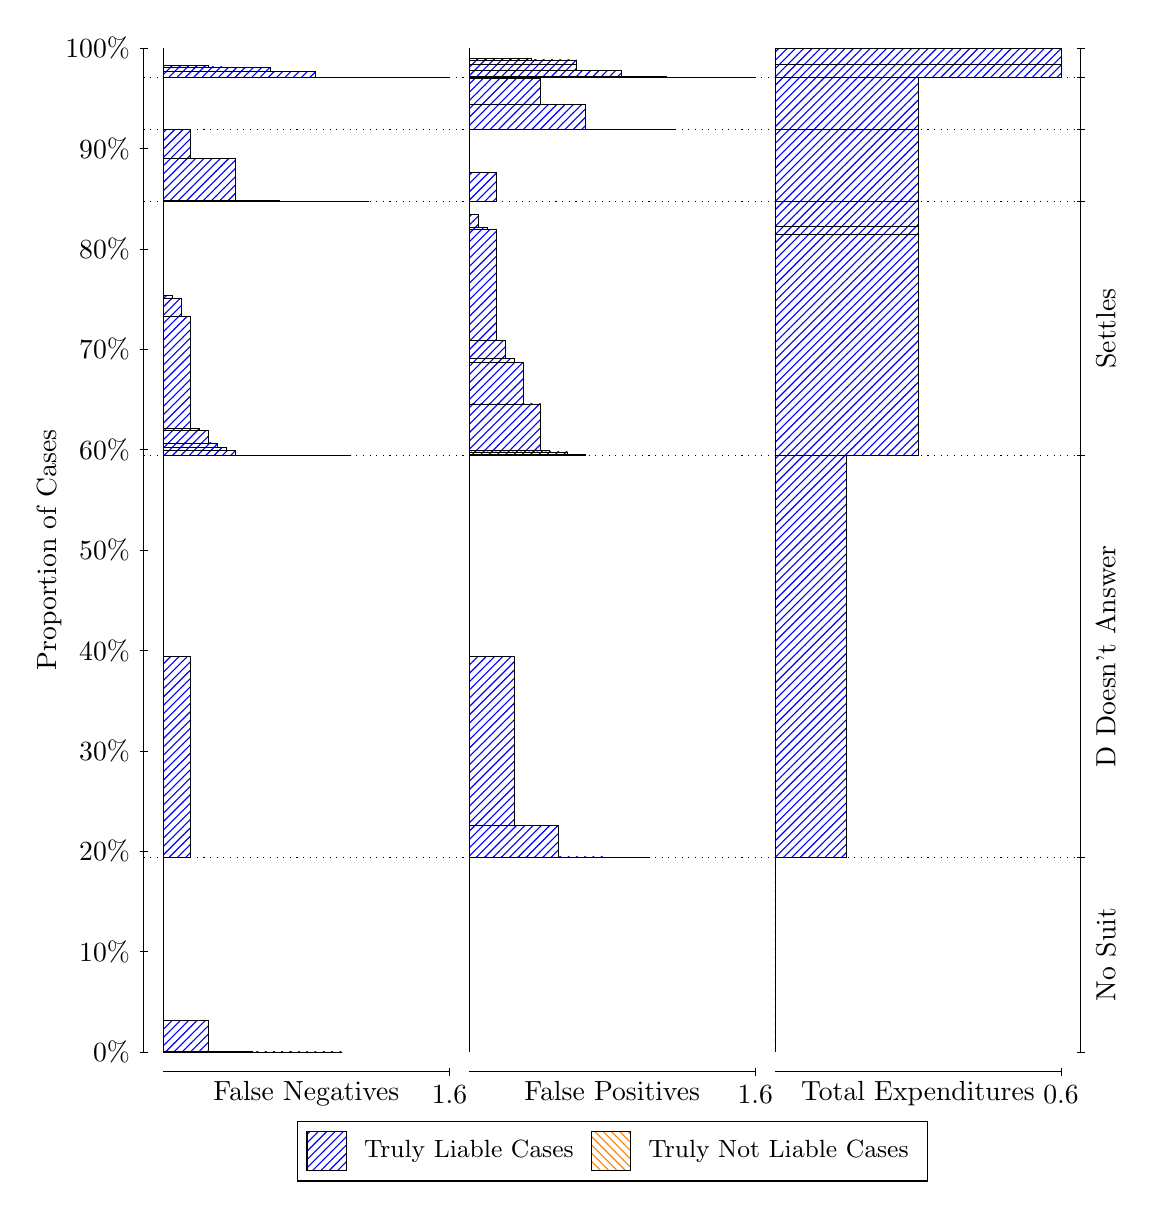
\begin{tikzpicture}
\draw[black, very thin] (1.5,1.75) -- (1.5,14.5);
\node[rotate=90, anchor=center] at (0.3, 8.125) {Proportion of Cases};
\draw[black, very thin] (1.45,1.75) -- (1.55,1.75);
\node[anchor=east] at (1.45, 1.75) {0\%};
\draw[black, very thin] (1.45,3.025) -- (1.55,3.025);
\node[anchor=east] at (1.45, 3.025) {10\%};
\draw[black, very thin] (1.45,4.3) -- (1.55,4.3);
\node[anchor=east] at (1.45, 4.3) {20\%};
\draw[black, very thin] (1.45,5.575) -- (1.55,5.575);
\node[anchor=east] at (1.45, 5.575) {30\%};
\draw[black, very thin] (1.45,6.85) -- (1.55,6.85);
\node[anchor=east] at (1.45, 6.85) {40\%};
\draw[black, very thin] (1.45,8.125) -- (1.55,8.125);
\node[anchor=east] at (1.45, 8.125) {50\%};
\draw[black, very thin] (1.45,9.4) -- (1.55,9.4);
\node[anchor=east] at (1.45, 9.4) {60\%};
\draw[black, very thin] (1.45,10.675) -- (1.55,10.675);
\node[anchor=east] at (1.45, 10.675) {70\%};
\draw[black, very thin] (1.45,11.95) -- (1.55,11.95);
\node[anchor=east] at (1.45, 11.95) {80\%};
\draw[black, very thin] (1.45,13.225) -- (1.55,13.225);
\node[anchor=east] at (1.45, 13.225) {90\%};
\draw[black, very thin] (1.45,14.5) -- (1.55,14.5);
\node[anchor=east] at (1.45, 14.5) {100\%};

\draw[black, very thin] (13.4,1.75) -- (13.4,14.5);
\draw[black, very thin] (13.35,1.75) -- (13.45,1.75);
\node[anchor=west] at (13.35, 1.75) {};
\draw[black, very thin] (13.35,4.2243) -- (13.45,4.2243);
\node[anchor=west] at (13.35, 4.2243) {};
\draw[black, very thin] (13.35,9.3219) -- (13.45,9.3219);
\node[anchor=west] at (13.35, 9.3219) {};
\draw[black, very thin] (13.35,12.552) -- (13.45,12.552);
\node[anchor=west] at (13.35, 12.552) {};
\draw[black, very thin] (13.35,13.465) -- (13.45,13.465);
\node[anchor=west] at (13.35, 13.465) {};
\draw[black, very thin] (13.35,14.126) -- (13.45,14.126);
\node[anchor=west] at (13.35, 14.126) {};
\draw[black, very thin] (13.35,14.5) -- (13.45,14.5);
\node[anchor=west] at (13.35, 14.5) {};

\draw[black, very thin, pattern color=blue, pattern=north east lines] (1.75,1.75) rectangle (4.0208,1.75);
\draw[black, very thin, pattern color=blue, pattern=north east lines] (1.75,1.75) rectangle (3.4531,1.75);
\draw[black, very thin, pattern color=blue, pattern=north east lines] (1.75,1.75) rectangle (2.8854,1.7535);
\draw[black, very thin, pattern color=blue, pattern=north east lines] (1.75,1.7535) rectangle (2.3177,2.1551);
\draw[black, very thin, pattern color=orange, pattern=north west lines] (1.75,2.1551) rectangle (1.75,2.1551);
\draw[black, very thin, pattern color=blue, pattern=north east lines] (1.75,2.1551) rectangle (1.75,4.2243);
\draw[black, very thin, pattern color=blue, pattern=north east lines] (1.75,4.2243) rectangle (2.0906,6.7701);
\draw[black, very thin, pattern color=orange, pattern=north west lines] (1.75,6.7701) rectangle (1.75,6.7701);
\draw[black, very thin, pattern color=blue, pattern=north east lines] (1.75,6.7701) rectangle (1.75,9.3219);
\draw[black, very thin, pattern color=blue, pattern=north east lines] (1.75,9.3219) rectangle (4.1344,9.3219);
\draw[black, very thin, pattern color=blue, pattern=north east lines] (1.75,9.3219) rectangle (3.9073,9.3219);
\draw[black, very thin, pattern color=blue, pattern=north east lines] (1.75,9.3219) rectangle (3.6802,9.3219);
\draw[black, very thin, pattern color=blue, pattern=north east lines] (1.75,9.3219) rectangle (3.5667,9.3219);
\draw[black, very thin, pattern color=blue, pattern=north east lines] (1.75,9.3219) rectangle (3.4531,9.3219);
\draw[black, very thin, pattern color=blue, pattern=north east lines] (1.75,9.3219) rectangle (3.3396,9.3219);
\draw[black, very thin, pattern color=blue, pattern=north east lines] (1.75,9.3219) rectangle (3.226,9.3219);
\draw[black, very thin, pattern color=blue, pattern=north east lines] (1.75,9.3219) rectangle (3.1125,9.322);
\draw[black, very thin, pattern color=blue, pattern=north east lines] (1.75,9.322) rectangle (2.999,9.3234);
\draw[black, very thin, pattern color=blue, pattern=north east lines] (1.75,9.3234) rectangle (2.8854,9.3237);
\draw[black, very thin, pattern color=blue, pattern=north east lines] (1.75,9.3237) rectangle (2.7719,9.325);
\draw[black, very thin, pattern color=blue, pattern=north east lines] (1.75,9.325) rectangle (2.6583,9.3862);
\draw[black, very thin, pattern color=blue, pattern=north east lines] (1.75,9.3862) rectangle (2.5448,9.4274);
\draw[black, very thin, pattern color=blue, pattern=north east lines] (1.75,9.4274) rectangle (2.4312,9.4843);
\draw[black, very thin, pattern color=blue, pattern=north east lines] (1.75,9.4843) rectangle (2.3177,9.6479);
\draw[black, very thin, pattern color=blue, pattern=north east lines] (1.75,9.6479) rectangle (2.2042,9.6726);
\draw[black, very thin, pattern color=blue, pattern=north east lines] (1.75,9.6726) rectangle (2.0906,11.089);
\draw[black, very thin, pattern color=blue, pattern=north east lines] (1.75,11.089) rectangle (1.9771,11.318);
\draw[black, very thin, pattern color=blue, pattern=north east lines] (1.75,11.318) rectangle (1.8635,11.363);
\draw[black, very thin, pattern color=orange, pattern=north west lines] (1.75,11.363) rectangle (1.75,11.363);
\draw[black, very thin, pattern color=blue, pattern=north east lines] (1.75,11.363) rectangle (1.75,12.552);
\draw[black, very thin, pattern color=blue, pattern=north east lines] (1.75,12.552) rectangle (4.3615,12.552);
\draw[black, very thin, pattern color=blue, pattern=north east lines] (1.75,12.552) rectangle (3.7937,12.552);
\draw[black, very thin, pattern color=blue, pattern=north east lines] (1.75,12.552) rectangle (3.226,12.568);
\draw[black, very thin, pattern color=blue, pattern=north east lines] (1.75,12.568) rectangle (2.6583,13.099);
\draw[black, very thin, pattern color=blue, pattern=north east lines] (1.75,13.099) rectangle (2.0906,13.465);
\draw[black, very thin, pattern color=orange, pattern=north west lines] (1.75,13.465) rectangle (1.75,13.465);
\draw[black, very thin, pattern color=blue, pattern=north east lines] (1.75,13.465) rectangle (2.0906,13.469);
\draw[black, very thin, pattern color=orange, pattern=north west lines] (1.75,13.469) rectangle (1.75,13.469);
\draw[black, very thin, pattern color=blue, pattern=north east lines] (1.75,13.469) rectangle (1.75,14.126);
\draw[black, very thin, pattern color=blue, pattern=north east lines] (1.75,14.126) rectangle (5.3833,14.126);
\draw[black, very thin, pattern color=blue, pattern=north east lines] (1.75,14.126) rectangle (4.8156,14.126);
\draw[black, very thin, pattern color=blue, pattern=north east lines] (1.75,14.126) rectangle (4.2479,14.131);
\draw[black, very thin, pattern color=blue, pattern=north east lines] (1.75,14.131) rectangle (3.6802,14.201);
\draw[black, very thin, pattern color=blue, pattern=north east lines] (1.75,14.201) rectangle (3.4531,14.201);
\draw[black, very thin, pattern color=blue, pattern=north east lines] (1.75,14.201) rectangle (3.1125,14.259);
\draw[black, very thin, pattern color=blue, pattern=north east lines] (1.75,14.259) rectangle (2.8854,14.259);
\draw[black, very thin, pattern color=blue, pattern=north east lines] (1.75,14.259) rectangle (2.5448,14.261);
\draw[black, very thin, pattern color=blue, pattern=north east lines] (1.75,14.261) rectangle (2.3177,14.277);
\draw[black, very thin, pattern color=blue, pattern=north east lines] (1.75,14.277) rectangle (1.9771,14.277);
\draw[black, very thin, pattern color=orange, pattern=north west lines] (1.75,14.277) rectangle (1.75,14.277);
\draw[black, very thin, pattern color=blue, pattern=north east lines] (1.75,14.277) rectangle (1.75,14.5);
\draw[black, very thin, pattern color=orange, pattern=north west lines] (5.6333,1.75) rectangle (5.6333,1.75);
\draw[black, very thin, pattern color=blue, pattern=north east lines] (5.6333,1.75) rectangle (5.6333,4.2243);
\draw[black, very thin, pattern color=orange, pattern=north west lines] (5.6333,4.2243) rectangle (7.9042,4.2243);
\draw[black, very thin, pattern color=blue, pattern=north east lines] (5.6333,4.2243) rectangle (7.9042,4.2243);
\draw[black, very thin, pattern color=blue, pattern=north east lines] (5.6333,4.2243) rectangle (7.3365,4.2272);
\draw[black, very thin, pattern color=blue, pattern=north east lines] (5.6333,4.2272) rectangle (6.7687,4.6312);
\draw[black, very thin, pattern color=blue, pattern=north east lines] (5.6333,4.6312) rectangle (6.201,6.7761);
\draw[black, very thin, pattern color=blue, pattern=north east lines] (5.6333,6.7761) rectangle (5.6333,9.3219);
\draw[black, very thin, pattern color=orange, pattern=north west lines] (5.6333,9.3219) rectangle (7.1094,9.3219);
\draw[black, very thin, pattern color=blue, pattern=north east lines] (5.6333,9.3219) rectangle (7.1094,9.3428);
\draw[black, very thin, pattern color=orange, pattern=north west lines] (5.6333,9.3428) rectangle (6.8823,9.3428);
\draw[black, very thin, pattern color=blue, pattern=north east lines] (5.6333,9.3428) rectangle (6.8823,9.372);
\draw[black, very thin, pattern color=orange, pattern=north west lines] (5.6333,9.372) rectangle (6.6552,9.372);
\draw[black, very thin, pattern color=blue, pattern=north east lines] (5.6333,9.372) rectangle (6.6552,9.387);
\draw[black, very thin, pattern color=blue, pattern=north east lines] (5.6333,9.387) rectangle (6.5417,9.98);
\draw[black, very thin, pattern color=orange, pattern=north west lines] (5.6333,9.98) rectangle (6.4281,9.98);
\draw[black, very thin, pattern color=blue, pattern=north east lines] (5.6333,9.98) rectangle (6.4281,9.9819);
\draw[black, very thin, pattern color=blue, pattern=north east lines] (5.6333,9.9819) rectangle (6.3146,10.511);
\draw[black, very thin, pattern color=orange, pattern=north west lines] (5.6333,10.511) rectangle (6.201,10.511);
\draw[black, very thin, pattern color=blue, pattern=north east lines] (5.6333,10.511) rectangle (6.201,10.556);
\draw[black, very thin, pattern color=blue, pattern=north east lines] (5.6333,10.556) rectangle (6.0875,10.785);
\draw[black, very thin, pattern color=blue, pattern=north east lines] (5.6333,10.785) rectangle (5.974,12.201);
\draw[black, very thin, pattern color=blue, pattern=north east lines] (5.6333,12.201) rectangle (5.8604,12.226);
\draw[black, very thin, pattern color=blue, pattern=north east lines] (5.6333,12.226) rectangle (5.7469,12.39);
\draw[black, very thin, pattern color=blue, pattern=north east lines] (5.6333,12.39) rectangle (5.6333,12.552);
\draw[black, very thin, pattern color=orange, pattern=north west lines] (5.6333,12.552) rectangle (5.974,12.552);
\draw[black, very thin, pattern color=blue, pattern=north east lines] (5.6333,12.552) rectangle (5.974,12.917);
\draw[black, very thin, pattern color=blue, pattern=north east lines] (5.6333,12.917) rectangle (5.6333,13.465);
\draw[black, very thin, pattern color=orange, pattern=north west lines] (5.6333,13.465) rectangle (8.2448,13.465);
\draw[black, very thin, pattern color=blue, pattern=north east lines] (5.6333,13.465) rectangle (8.2448,13.465);
\draw[black, very thin, pattern color=blue, pattern=north east lines] (5.6333,13.465) rectangle (7.6771,13.468);
\draw[black, very thin, pattern color=blue, pattern=north east lines] (5.6333,13.468) rectangle (7.1094,13.788);
\draw[black, very thin, pattern color=blue, pattern=north east lines] (5.6333,13.788) rectangle (6.5417,14.122);
\draw[black, very thin, pattern color=blue, pattern=north east lines] (5.6333,14.122) rectangle (5.974,14.126);
\draw[black, very thin, pattern color=orange, pattern=north west lines] (5.6333,14.126) rectangle (9.2667,14.126);
\draw[black, very thin, pattern color=blue, pattern=north east lines] (5.6333,14.126) rectangle (9.2667,14.126);
\draw[black, very thin, pattern color=orange, pattern=north west lines] (5.6333,14.126) rectangle (8.699,14.126);
\draw[black, very thin, pattern color=blue, pattern=north east lines] (5.6333,14.126) rectangle (8.699,14.127);
\draw[black, very thin, pattern color=orange, pattern=north west lines] (5.6333,14.127) rectangle (8.1313,14.127);
\draw[black, very thin, pattern color=blue, pattern=north east lines] (5.6333,14.127) rectangle (8.1313,14.135);
\draw[black, very thin, pattern color=blue, pattern=north east lines] (5.6333,14.135) rectangle (7.5635,14.219);
\draw[black, very thin, pattern color=orange, pattern=north west lines] (5.6333,14.219) rectangle (7.5635,14.219);
\draw[black, very thin, pattern color=blue, pattern=north east lines] (5.6333,14.219) rectangle (7.5635,14.22);
\draw[black, very thin, pattern color=blue, pattern=north east lines] (5.6333,14.22) rectangle (6.9958,14.29);
\draw[black, very thin, pattern color=blue, pattern=north east lines] (5.6333,14.29) rectangle (6.9958,14.349);
\draw[black, very thin, pattern color=orange, pattern=north west lines] (5.6333,14.349) rectangle (6.7687,14.349);
\draw[black, very thin, pattern color=blue, pattern=north east lines] (5.6333,14.349) rectangle (6.7687,14.349);
\draw[black, very thin, pattern color=blue, pattern=north east lines] (5.6333,14.349) rectangle (6.4281,14.35);
\draw[black, very thin, pattern color=blue, pattern=north east lines] (5.6333,14.35) rectangle (6.4281,14.365);
\draw[black, very thin, pattern color=orange, pattern=north west lines] (5.6333,14.365) rectangle (6.201,14.365);
\draw[black, very thin, pattern color=blue, pattern=north east lines] (5.6333,14.365) rectangle (6.201,14.368);
\draw[black, very thin, pattern color=blue, pattern=north east lines] (5.6333,14.368) rectangle (5.8604,14.368);
\draw[black, very thin, pattern color=blue, pattern=north east lines] (5.6333,14.368) rectangle (5.8604,14.368);
\draw[black, very thin, pattern color=orange, pattern=north west lines] (5.6333,14.368) rectangle (5.6333,14.368);
\draw[black, very thin, pattern color=blue, pattern=north east lines] (5.6333,14.368) rectangle (5.6333,14.5);
\draw[black, very thin, pattern color=orange, pattern=north west lines] (9.5167,1.75) rectangle (9.5167,1.75);
\draw[black, very thin, pattern color=blue, pattern=north east lines] (9.5167,1.75) rectangle (9.5167,4.2243);
\draw[black, very thin, pattern color=orange, pattern=north west lines] (9.5167,4.2243) rectangle (10.425,4.2243);
\draw[black, very thin, pattern color=blue, pattern=north east lines] (9.5167,4.2243) rectangle (10.425,9.3219);
\draw[black, very thin, pattern color=orange, pattern=north west lines] (9.5167,9.3219) rectangle (11.333,9.3219);
\draw[black, very thin, pattern color=blue, pattern=north east lines] (9.5167,9.3219) rectangle (11.333,12.135);
\draw[black, very thin, pattern color=orange, pattern=north west lines] (9.5167,12.135) rectangle (11.333,12.135);
\draw[black, very thin, pattern color=blue, pattern=north east lines] (9.5167,12.135) rectangle (11.333,12.239);
\draw[black, very thin, pattern color=orange, pattern=north west lines] (9.5167,12.239) rectangle (11.333,12.239);
\draw[black, very thin, pattern color=blue, pattern=north east lines] (9.5167,12.239) rectangle (11.333,12.552);
\draw[black, very thin, pattern color=orange, pattern=north west lines] (9.5167,12.552) rectangle (11.333,12.552);
\draw[black, very thin, pattern color=blue, pattern=north east lines] (9.5167,12.552) rectangle (11.333,13.465);
\draw[black, very thin, pattern color=orange, pattern=north west lines] (9.5167,13.465) rectangle (11.333,13.465);
\draw[black, very thin, pattern color=blue, pattern=north east lines] (9.5167,13.465) rectangle (11.333,14.126);
\draw[black, very thin, pattern color=orange, pattern=north west lines] (9.5167,14.126) rectangle (13.15,14.126);
\draw[black, very thin, pattern color=blue, pattern=north east lines] (9.5167,14.126) rectangle (13.15,14.289);
\draw[black, very thin, pattern color=orange, pattern=north west lines] (9.5167,14.289) rectangle (13.15,14.289);
\draw[black, very thin, pattern color=blue, pattern=north east lines] (9.5167,14.289) rectangle (13.15,14.5);
\draw[black, dotted] (1.5,4.2243) -- (13.4,4.2243);
\draw[black, dotted] (1.5,9.3219) -- (13.4,9.3219);
\draw[black, dotted] (1.5,12.552) -- (13.4,12.552);
\draw[black, dotted] (1.5,13.465) -- (13.4,13.465);
\draw[black, dotted] (1.5,14.126) -- (13.4,14.126);
\draw[black, very thin] (1.75,1.5) -- (5.3833,1.5);
\node[anchor=north] at (3.5667, 1.5) {False Negatives};
\draw[black, very thin] (5.3833,1.45) -- (5.3833,1.55);
\node[anchor=north] at (5.3833, 1.45) {1.6};

\draw[black, very thin] (5.6333,1.5) -- (9.2667,1.5);
\node[anchor=north] at (7.45, 1.5) {False Positives};
\draw[black, very thin] (9.2667,1.45) -- (9.2667,1.55);
\node[anchor=north] at (9.2667, 1.45) {1.6};

\draw[black, very thin] (9.5167,1.5) -- (13.15,1.5);
\node[anchor=north] at (11.333, 1.5) {Total Expenditures};
\draw[black, very thin] (13.15,1.45) -- (13.15,1.55);
\node[anchor=north] at (13.15, 1.45) {0.6};

\node[black, centered, rotate=90] at (13.72, 2.9871) {No Suit};
\node[black, centered, rotate=90] at (13.72, 6.7731) {D Doesn't Answer};
\node[black, centered, rotate=90] at (13.72, 10.937) {Settles};




\draw (7.449999999999999,1.5) node[draw=none] (baseCoordinate) {};
\begin{scope}[align=center]
        \matrix[scale=0.5, draw=black, below=0.5cm of baseCoordinate, nodes={draw}, column sep=0.1cm]{
            \node[rectangle, draw, minimum width=0.5cm, minimum height=0.5cm, pattern=north east lines, pattern color=blue] {}; &
            \node[draw=none, font=\small] (B) {Truly Liable Cases}; &
            \node[rectangle, draw, minimum width=0.5cm, minimum height=0.5cm, pattern=north west lines, pattern color=orange] {}; &
            \node[draw=none, font=\small] (B) {Truly Not Liable Cases}; \\
            };
\end{scope}

\end{tikzpicture}
\end{document}